\subsection{Знаходження матриці гомографії за допомогою RANSAC}

Матриця гомографії ~---~ матриця, що описує зв'язок точок між двома зображеннями плоскої поверхні.

\begin{equation}
    H =
    \begin{bmatrix}
        h_{11} & h_{12} & h_{13} \\
        h_{21} & h_{22} & h_{13} \\
        h_{31} & h_{32} & h_{33}
    \end{bmatrix}
    \label{eq:h_matrix}
\end{equation}

\begin{equation}
    H^{i} \cdot p_{j}^{i + s} = c \cdot p_{j}^{i},\quad\forall i = \overline{1,4\ }
    \label{eq:h_connection}
\end{equation}
Рівняння \eqref{eq:h_connection} можна легко розв'язати відносно невідомої матриці
\(H^{i}\). Цю матрицю можна використати для компенсації руху камери
~---~ ми застосовуємо її до координат пікселів кадру номер \(i + s\), після
чого точки зображення, отриманого в результаті перетворення, мають ті ж
координати, що й відповідні їм точки на кадрі під номером \(i\). Якщо
отримані координати не цілочисельні, їх можна округлити, що не матиме
значного негативного впливу на якість результату.

Знаходження $H$ вимагає знаходження всіх 9 параметрів матриці \eqref{eq:h_matrix}.
Візьмемо пару відповідних точок $T$ та $T'$: $T = ((x_1,y_1,1), (x_2,y_2,1),
    (x_3,y_3,1), (x_4,y_4,1)), T' = ((x'_1,y'_1,1), (x'_2,y'_2,1), (x'_3,y'_3,1), (x'_4,y'_4,1))$.
Перепишемо \eqref{eq:h_connection} у матричній формі для $T$ та $T'$.
\begin{equation}
    \begin{bmatrix}
        x'_i\lambda \\
        y'_i\lambda \\
        \lambda
    \end{bmatrix}
    =
    \begin{bmatrix}
        h_{11} & h_{12} & h_{13} \\
        h_{21} & h_{22} & h_{13} \\
        h_{31} & h_{32} & h_{33}
    \end{bmatrix}
    \begin{bmatrix}
        x_i \\
        y_i \\
        1
    \end{bmatrix}
    ,\quad\forall i,j = \overline{1,4\ }
    \label{eq:h_connection2}
\end{equation}
приходимо до розв'язку системи
\begin{equation*}
    \underbrace{
        \begin{bmatrix}
            x_1 & y_1 & 1 & 0   & 0   & 0 & -x_1x'_1 -y_1x'_1 \\
            x_2 & y_2 & 1 & 0   & 0   & 0 & -x_2x'_2 -y_2x'_2 \\
            x_3 & y_3 & 1 & 0   & 0   & 0 & -x_3x'_3 -y_3x'_3 \\
            x_4 & y_4 & 1 & 0   & 0   & 0 & -x_4x'_4 -y_4x'_4 \\
            0   & 0   & 0 & x_1 & y_1 & 1 & -x_1y'_1 -y_1y'_1 \\
            0   & 0   & 0 & x_2 & y_2 & 1 & -x_2y'_2 -y_2y'_2 \\
            0   & 0   & 0 & x_3 & y_3 & 1 & -x_3y'_3 -y_3y'_3 \\
            0   & 0   & 0 & x_4 & y_4 & 1 & -x_4y'_4 -y_4y'_4
        \end{bmatrix}
    }_\textrm{A}
    \begin{bmatrix}
        h_{11} \\
        h_{12} \\
        h_{13} \\
        h_{21} \\
        h_{22} \\
        h_{23} \\
        h_{31} \\
        h_{32}
    \end{bmatrix}
    =
    h_{33}
    \begin{bmatrix}
        x'_1 \\
        x'_2 \\
        x'_3 \\
        x'_4 \\
        y'_1 \\
        y'_2 \\
        y'_3 \\
        y'_4
    \end{bmatrix}.
\end{equation*}
Варто відмітити, що ми потім позбуваємось $h_{33}$, щоб $H$ була нормованою, оскільки вона
зв'язує точки площин, в яких 3-тя координата одиниця.
У $A$ маємо 8 рівнянь, для знаходження параметрів яких потрібно, щоб $A$ була повноранговою.
Для отримання $H$ застосовується сингулярний розклад (SVD) матриці $А = U\Sigma V^*$.
Після розкладу $V^*$ має розмір $9\times9$. Параметри $H$ знаходяться в останньому рядку $V^*$.

\begin{equation}
    H = V^{*}_{9,\cdot }/V^{*}_{9,9},\quad H \in R^{1 \times 9} \rightarrow H \in R^{3 \times 3}
    \label{eq:honography_svd}
\end{equation}

Для оцінки гомографії використали принцип RANSAC \cite{bib:ransac} (алгоритм \ref{al:ransac_homography}).
Користувач вводить рівень \(\varepsilon > 0\)
дозволеної похибки розрахунків ~---~ що менше, то краще, проте тим довше
буде працювати алгоритм пошуку матриці гомографії
\begin{equation}
    E(H) = \sum_{(x,x') \in M^{i,i+s}}
    \left\llbracket \left\lVert
    \frac{H\cdot x'}{(H\cdot x')_z} - x
    \right\rVert \leq \varepsilon
    \right\rrbracket
    \to \max\limits_{\substack{H \in \mathbb{R}^{3 \times 3} \\ \det{H} \neq 0}}.
    \label{eq:homography_estimation}
\end{equation}

\begin{algorithm}[H]
    \caption{Алгоритм знаходження гомографії за принципом RANSAC}
    \label{al:ransac_homography}
    \begin{algorithmic}
        \State \textbf{Вхід:} $M^{i,i+s}$ - множина відповідних точок, $\varepsilon$ та $n$ - кількість ітерацій.
        \State \textbf{Вихід:} $H^{best}$ - найкраща матриця гомографії.
        \State $\forall i = \overline{1,n}$
        \State \quad 1. Вибираємо випадковим чином 4 пари відповідних точок $T$ та $T'$ з $M^{i,i+s}$.
        \State \quad 2. Обчислюємо $H$ по формулі \eqref{eq:honography_svd}
        \State \quad 3. Обчислюємо $E(H)$ по формулі \eqref{eq:homography_estimation}
        \State \quad 4. Якщо  $E(H) < E(H^{best})$:
        \State \qquad $H^{best} \gets H$
    \end{algorithmic}
\end{algorithm}

\subsubsection{Обробка ключових точок з маскою}

Ключові точки (рис. \ref{fig:yakovlev:keypoints:a}), що дає нам дескриптор ознак SIFT, ми
використовуємо для оцінки гомографії, але також видаляємо ті ключові
точки, які потрапляють в область маски рухомих об'єктів.
Таким чином, ми зменшуємо ймовірність того, що замість дошки алгоритм ``зачепиться'' за одяг
викладача (рис. \ref{fig:matches_img}) або інші рухомі об'єкти.
На рис. \ref{fig:yakovlev:keypoints:b} можна помітити, що
існують точки, які насправді не належать рухомим об'єктам кадру
\(F^{i + s}\), але були видалені. Це відбулось через те, що такі точки
відповідають точкам з кадру \(F^{i}\), які в свою чергу лежать в межах маски рухомих об'єктів.

\begin{figure}[H]
    \centering
    \begin{subfigure}[b]{0.55\textwidth}
        \centering
        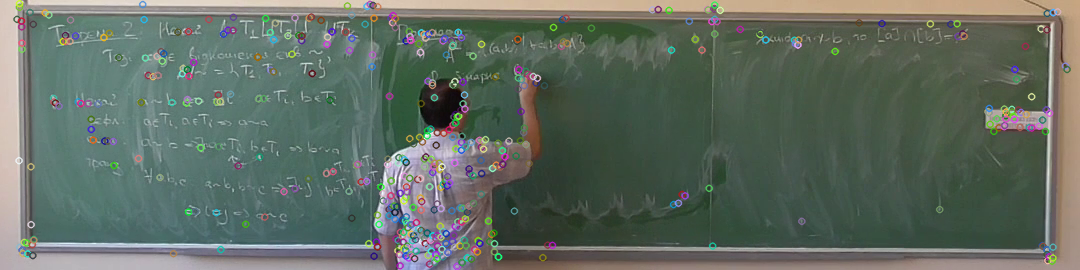
\includegraphics[width=\textwidth]{images/next_frame_kp}
        \caption{Ключові точки на кадрі $F^{i+s}$
            \label{fig:yakovlev:keypoints:a}
        }
    \end{subfigure}
    \begin{subfigure}[b]{0.55\textwidth}
        \centering
        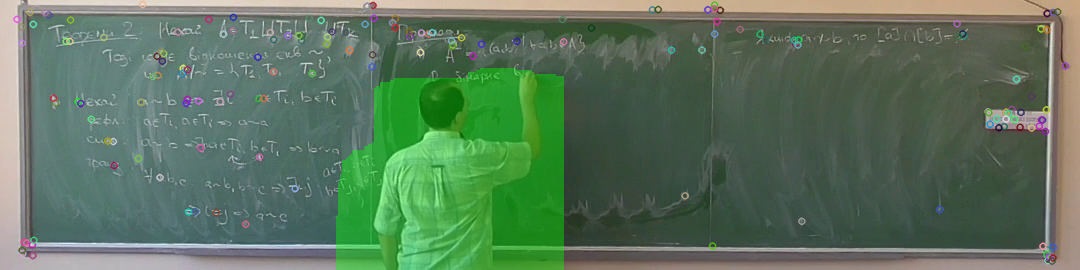
\includegraphics[width=\textwidth]{images/next_frame_matches_mask}
        \caption{Відповідні ключові точки на кадрі $F^{i+s}$, що залишились після
            видалення тих точок, що потрапили в область маски рухомих
            об'єктів
            \label{fig:yakovlev:keypoints:b}
        }
    \end{subfigure}
    \caption{Результат застосування маски для відповідних точок з відео \cite{video:mmzi:yakovlev_discrete_math}
        \label{fig:yakovlev:keypoints}
    }
\end{figure}
